\section{Benchmark NIST-12 "Multiple Difficulties"}
\label{sec:bench-12}

The solution to this problem combines four types of benchmarks 
seen in previous sections into the same problem, 
where the wave front intersects the boundary
layer and corner singularity, and the peak is centered on the wave front.
%It contains a point singularity due to a reentrant corner, a circular wave front (which might
%include a singularity at the center of the circle), a sharp peak, and a boundary layer.
The equation solved is the Poisson's equation. 

\begin{equation} \label{multiple}
-\Delta u = f
\end{equation}

in the L-shaped domain, equipped with Dirichlet boundary conditions
given by the exact solution.
The exact solution:

\begin{equation}\label{exact-nist-12}
u(x,y) =  r^{\alpha_{C} }\sin(\alpha_{C} \theta)
+ e^{-\alpha_{P} ((x - x_{P})^{2} + (y - y_{P})^{2})}
+ tan^{-1}(\alpha_{W} (r_{W} - r_{0}))
+ e^{-(1 - y) / \epsilon}
\end{equation}

where $\alpha_C = \pi / \omega_C$, $r = \sqrt{x^2+y^2}$
and $\theta = tan^{-1}(y/x)$, here $\omega_C$ determines
the angle of the re-entrant corner.
$(x_{P}, y_{P})$ is the location of the peak, $\alpha$
determines the strength of the peak. Furthermore
$r_{W} = \sqrt{(x - x_{W})^{2} + (y - y_{W})^{2}}$,
where $(x_{W}, y_{W})$ is the center of the circular wave front,
$r_{0}$ is the distance from the wave front to the
center of the circle, and $\alpha_W$ gives
the steepness of the wave front. The parameter $\epsilon$ determines the
strength of the boundary layer, the boundary layer was placed on $y = -1$.
The right-hand side $f$ is calculated by inserting (\ref{exact-nist-12})
into (\ref{multiple}).
The solution of NIST-12 with $\omega_C = 3 \pi /2$,
$(x_{W}, y_{W}) = (0, -3/4)$, $r_{0} = 3/4$, $\alpha_{W} = 200$,
$(x_{P}, y_{P}) = (\sqrt{5} / 4, -1/4)$,
$\epsilon = 1/100$ is shown in Fig. \ref{fig:sln-nist12}.

\begin{figure}[!ht]
\centering
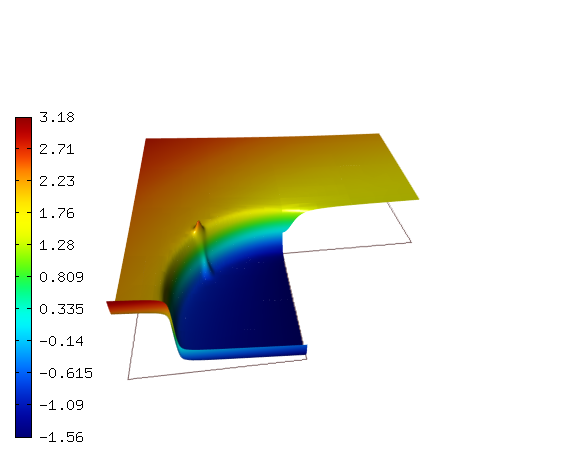
\includegraphics[height=5cm]{nist/nist-12/solution.png}
\caption{The solution to NIST-12 benchmark problem.}
\label{fig:sln-nist12}
\end{figure}

The goal of the benchmark is to reach a relative error below
$10^{-1}$~\% in the $H^1$-norm with as few DOFs as possible.
We begin with adaptive $hp$-FEM,
the initial mesh is shown in Fig. \ref{fig:nist-12-hp-aniso} (left).
After 26 adaptivity steps, the resulting mesh with 4438 DOF is shown
in Fig. \ref{fig:nist-12-hp-aniso} (right).

\begin{figure}[!ht]
\centering
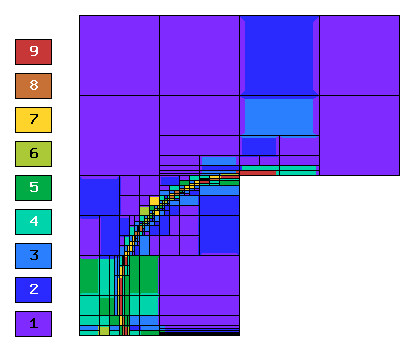
\includegraphics[height=5cm]{nist/nist-12/mesh_hp_aniso_init.png}\ \
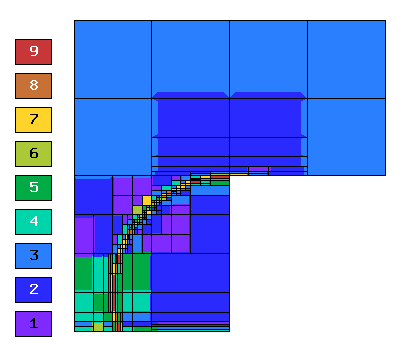
\includegraphics[height=5cm]{nist/nist-12/mesh_hp_aniso.png}
\caption{Initial mesh (left) and final mesh (right) for $hp$-FEM with anisotropic refinements.}
\label{fig:nist-12-hp-aniso}
\end{figure}

The final relative error estimate in $H^1$-norm was 9.85118e-01 \%,
and it was identical to the exact error in all printed digits.
We also solved this benchmark with adaptive $h$-FEM
with linear (left) and quadratic (right)
elements, with anisotropic refinements enabled.
Final meshes for the $h$-FEM computations are shown
in Fig. \ref{fig:nist-12-h-aniso}.

\begin{figure}[!ht]
\centering
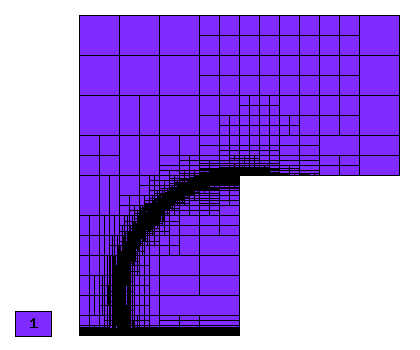
\includegraphics[height=5cm]{nist/nist-12/mesh_h1_aniso.png}\ \
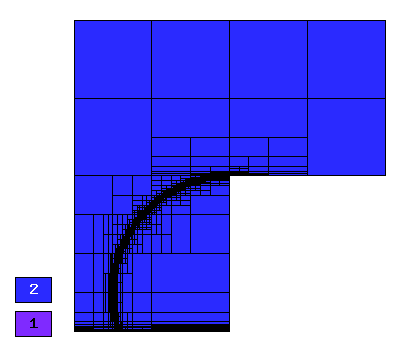
\includegraphics[height=5cm]{nist/nist-12/mesh_h2_aniso.png}
\caption{Final mesh for $h$-FEM anisotropic refinements with linear and quadratic elements.}
\label{fig:nist-12-h-aniso}
\end{figure}

Finally, Figs. \ref{fig:nist-12-conv} compare all
three approaches to automatic adaptivity from the point
of view of DOF and CPU convergence.

\begin{figure}[!ht]
\centering
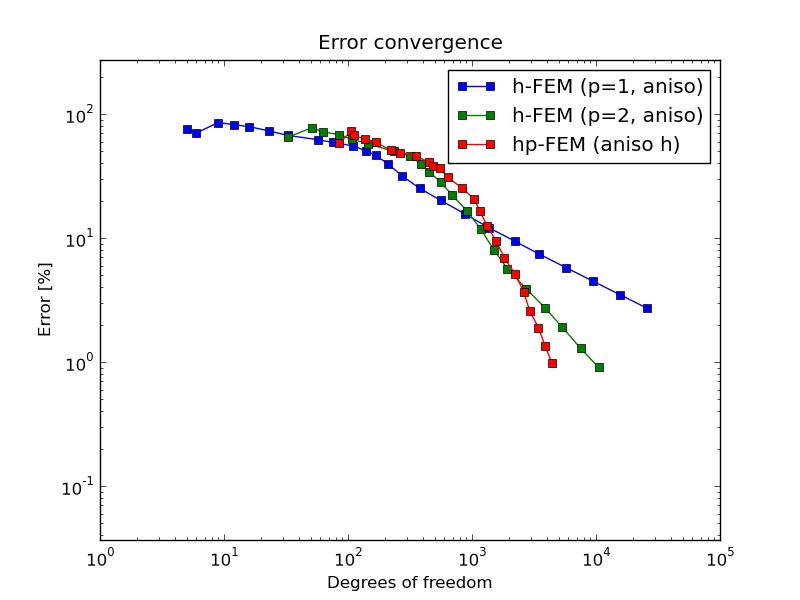
\includegraphics[height=5cm]{nist/nist-12/conv_dof_aniso.png}\ \
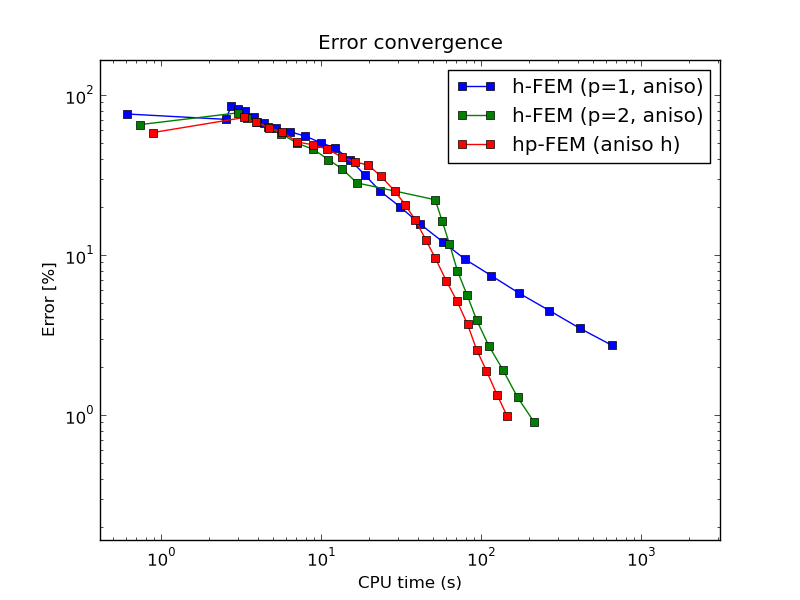
\includegraphics[height=5cm]{nist/nist-12/conv_cpu_aniso.png}
\caption{DOF and CPU time convergence graphs.}
\label{fig:nist-12-conv}
\end{figure}

